\section{Web Application}
%% (Reihenfolge noch vorläufig)
%% - Was ist Django?
%% - Wie setzt Django das MVC-Pattern um?
%% - Installation einschließlich Dependencies
%% - Benutzung der App (allgemein und Admin-Interface)
%% - Deployment
%% - Datenmodell (Ähnlichkeiten / Unterschiede zum XML-Schema)
%% - Zukünftige Erweiterungen (Templates und Views für Endnutzer,
%%   XML-Export, MySQL/Postgres backend)

\emph{Author: Tim Krones} \\

In addition to functionality for extracting and annotating the
contents of the Sbr-Regesten, the package also provides the basic
architecture for a web application. This chapter gives an overview of
the Django Framework for developing web application. It then describes
how to

\begin{itemize}
\item install necessary dependencies
\item run the application
\item use the admin interface to add or change data
\end{itemize}

and provides basic pointers for extending and deploying the
application. Also included is a detailed description of the data model
used for storing information extracted from the Sbr-Regesten in the
database associated with the application.

\subsection{The Django Web Framework}
\label{sec:django}

The information in this section is based on the official Django
documentation which can be found at
\url{https://docs.djangoproject.com/}.

Django is a Python Framework for rapid prototyping and development of
interactive web applications. It uses the MVC pattern to separate the
different tasks that are involved in creating interactive web
applications.

\subsubsection{The MVC Pattern}
\label{sec:mvc}

\href{https://en.wikipedia.org/wiki/Model_view_controller}{Model-View-Controller},
or MVC for short, is a
\href{https://en.wikipedia.org/wiki/Software_design_pattern}{Software Design Pattern}

commonly used by Web Frameworks such as Django and Ruby on Rails. The
basic idea of MVC is is to divide application logic into three layers.
The \emph{Model} layer is responsible for storing and operating on
data. This usually involves at least the basic
\href{https://en.wikipedia.org/wiki/CRUD}{CRUD} operations
\emph{Create}, \emph{Read}, \emph{Update}, and \emph{Delete}.The
\emph{View} layer takes care of presenting available data to end
users. \emph{Controllers} are responsible for handling user requests.
Depending on the type of request, this usually involves querying the
model layer for data, manipulating this data in various ways (if
necessary), and sending it off to the view layer for presentation.

Different frameworks interpret MVC in different ways; the next chapter
describes Django's implementation of this pattern.

\subsubsection{How Django Implements MVC}
\label{sec:django-mvc}

This chapter presents an overview of how Django interprets and
implements the MVC pattern. For an in-depth treatment of the
individual components, please consult the documentation at
\url{https://docs.djangoproject.com/}.

While Django's seperation of concerns is heavily influenced by the MVC
pattern conceptually, the framework uses a different terminology to
distinguish the individual components for dealing with (user)
requests, data, and presentation. The terminological differences tend
to confuse users that are new to Django or to working with MVC
frameworks in general, which makes it all the more important to
understand these differences before delving into Django development.

Django distinguishes between \emph{models}, \emph{templates}, and
\emph{views}, which is why the framework is commonly referred to as an
``MTV'' framework. The model layer in Django corresponds to the
concept of a model layer as it is defined (or at least commonly
understood) in the context of MVC. Django templates correspond to
views in MVC, and the responsibilities of Django views are similar to
those of controllers in MVC.

From an architectural point of view, a Django \emph{project} usually
consists of one or more Django \emph{apps}. Among other things, each
app includes a dedicated Python module for the model layer (called
\texttt{models.py}), two Python modules that are jointly responsible for
handling user requests (called \texttt{views.py} and \texttt{urls.py})
and a hierarchy of templates written in Django's template language.

The \texttt{models.py} module contains specialized Python classes
(called \emph{models}) which define the data model of a given Django
app. Each class corresponds to a table in the database of the project,
with additional tables being created as necessary to represent
relationships between different models.

The \texttt{views.py} module contains specialized Python functions
(called \emph{view functions}) for handling user requests. These
functions are responsible for querying the database for information,
manipulating that information if necessary, and rendering the
appropriate templates back to the user, filled with the information
that was requested. In this context, the \texttt{urls.py} module acts
as a kind of \emph{dispatcher}: It contains a mapping from URLs (or,
generally speaking, URL patterns) to appropriate view functions,
allowing Django to identify the actions it needs to take based on the
URL that was requested by the user.

\subsection{Installing and Using the Web Application}
\label{sec:webapp}

This chapter explains how to install and use the Sbr-Regesten Web
Application, and also provides some pointers on how to extend and
deploy it.

\subsubsection{Installation}
\label{sec:install}

\paragraph{Python and Django}
The Sbr-Regesten Web Application was developed using Python 2.7.3 and
Django 1.4.3.

Python binaries and source code for all major operating systems can be
obtained from \url{http://python.org/download/}. Python binaries are
usually pre-installed on Linux distributions, and different versions
can be obtained from standard repositories using a package manager:
Please note that at the time of this writing, Django is \textbf{not}
compatible with Python 3, so in order to run the app successfully,
Python 2.7.* needs to be installed.

The easiest way to install specific versions of Django is using the
\href{http://www.pip-installer.org/en/latest/}{pip-installer} which is
a tool for installing and managing Python packages. \texttt{pip}
should be available in the standard repositories of most Linux
distributions (package: python-pip). For generic installation
instructions, visit
\url{http://www.pip-installer.org/en/latest/installing.html}.

Once \texttt{pip} has been installed, version 1.4.3 of Django can be
installed using the following command:

\begin{verbatim}
$ pip install Django==1.4.3
\end{verbatim}

For instructions on how to install Django manually, consult
\href{https://www.djangoproject.com/download/}{this part} of the
Django documentation.

\paragraph{BeautifulSoup}
The process of extracting and annotating information from the
Sbr-Regesten makes heavy use of a tool called \emph{BeautifulSoup},
which needs to be installed in order to reproduce the extraction
process locally.

Like Django, BeautifulSoup is pip-installable:

\begin{verbatim}
$ pip install beautifulsoup4
\end{verbatim}

For the purpose of improving or extending the extraction process,
detailed information about BeautifulSoup can be found in its
\href{http://www.crummy.com/software/BeautifulSoup/bs4/doc/}{official documentation}.

\paragraph{Further Recommendations}
In addition to the hard dependencies described in the previous
sections, we recommend installing the \emph{IPython} interpreter as it
provides a lot of features not included in the standard python
interpreter and thus makes interacting with the database from Django's
development shell a lot easier. The latest version of IPython can be
installed using pip as follows:

\begin{verbatim}
$ pip install ipython
\end{verbatim}

\subsubsection{Running the Application}
\label{sec:run}

Once all necessary dependencies are installed, you are ready to run a
local instance of the application. Extract the contents of the source
archive to an appropriate folder in your file system and \texttt{cd}
into the root folder of the project. This folder is called
\texttt{sbr-regesten}. Look for a file called
\texttt{sbr-regesten.db}. If it's there, this means that source
package you have received includes a prepopulated database, and that
you can run the application right away by typing

\begin{verbatim}
$ python manage.py runserver
\end{verbatim}

If you find that the database file is missing from the source archive,
you need to proceed as follows: First, initialize the database by running

\begin{verbatim}
$ python manage.py syncdb
\end{verbatim}

At some point you will be asked whether or not you would like to
create a superuser for the database. Type \texttt{yes} and press
Enter, then provide a username, email address and password. For
development purposes it is both convenient and acceptable to simply
set username and password to \texttt{admin}.

When the \texttt{syncdb} command finishes, you can either start using
the application with an empty database by typing the
\texttt{runserver} command listed above, or you can go ahead and
populate the database with information from the Sbr-Regesten. Since
the extraction process was implemented as a Django \emph{management command},
you can trigger it using the following command:

\begin{verbatim}
$ python manage.py extract
\end{verbatim}

Note that this process might take a long time to finish.

\subsubsection{Using the Application}
\label{sec:use}

After starting the development server with the \texttt{runserver}
command, direct your browser to \url{http://127.0.0.1:8000/admin} to
access the application. You will be greeted by a login form:

\begin{figure}[h]
  \centering
  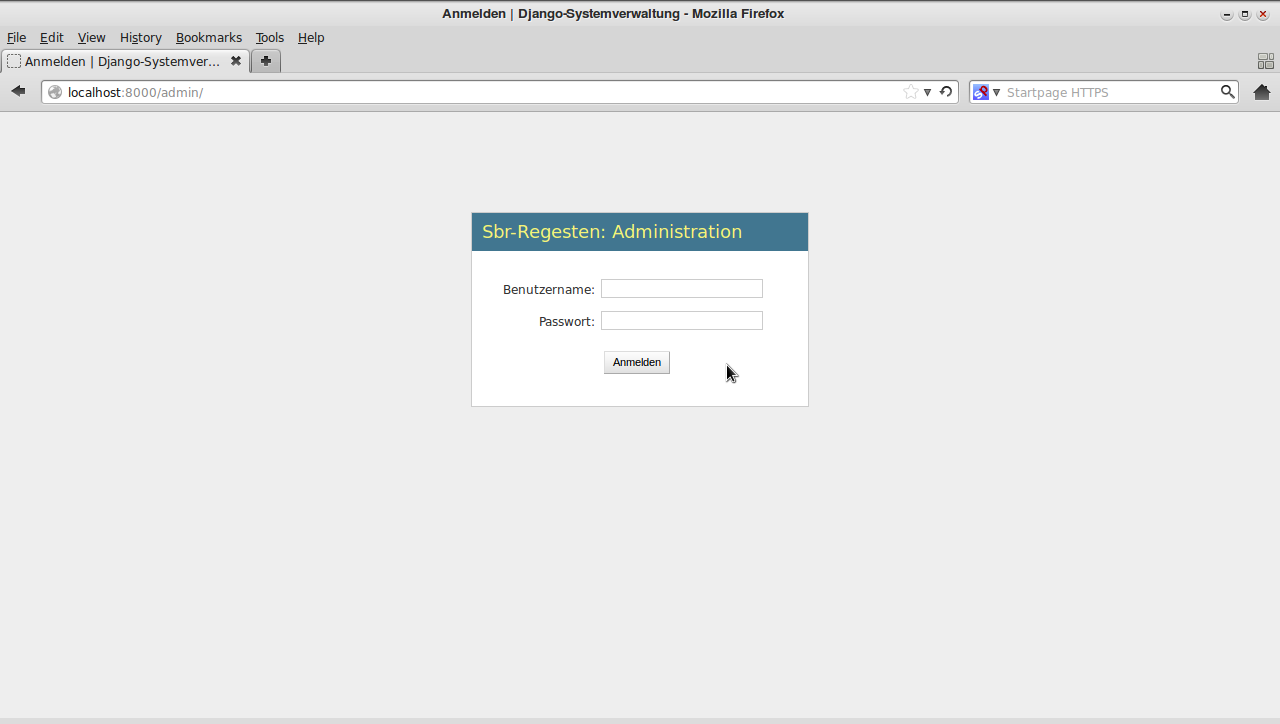
\includegraphics[scale=0.3]{img/admin-login}
  \caption{Login screen for the Django admin interface}
  \label{fig:admin-login}
\end{figure}

If you are working with a prepopulated database, enter \texttt{admin}
in both the \emph{Benutzername} and the \emph{Passwort} field. If you
initialized the database yourself, use the credentials you specified
in the \texttt{syncdb} step explained in the previous section.
Clicking on \emph{Anmelden} will take you to the main page of the
\emph{Django Admin Interface}:

\begin{figure}[h]
  \centering
  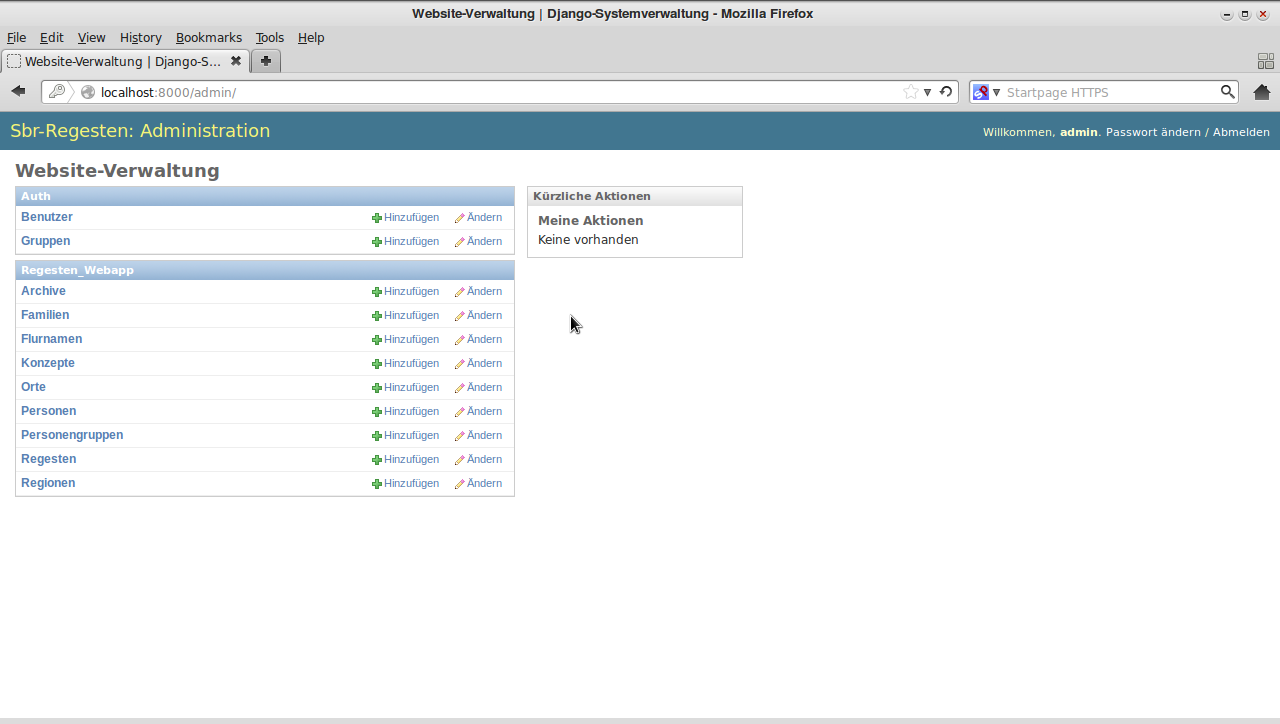
\includegraphics[scale=0.3]{img/admin-main}
  \caption{Main page of the admin interface, starting point for actions described below}
  \label{fig:admin-main}
\end{figure}

The admin interface allows you to browse, search and manipulate (i.e.
add, change, and delete) the data that is stored in the database from
the convenience of your browser.

\paragraph{Browsing and Searching Data}
From the main page of the admin interface you can get listings of
database entries for the following entities that can be found in the
Sbr-Regesten\footnote{Consult chapter \ref{sec:data-model} for more
  information about these entities.}:

\begin{itemize}
\item Archives (listed as \emph{Archive})
\item Families (listed as \emph{Familien})
\item Landmarks (listed as \emph{Flurnamen})
\item Concepts (listed as \emph{Konzepte})
\item Locations (listed as \emph{Orte})
\item Persons (listed as \emph{Personen})
\item Person groups (listed as \emph{Personengruppen})
\item Regests (listed as \emph{Regesten})
\item Regions (listed as \emph{Regionen})
\end{itemize}

Click on the name of a specific entity to get to the corresponding
listing of database entries. The listing for locations (\emph{Orte})
looks like this:

\begin{figure}[h]
  \centering
  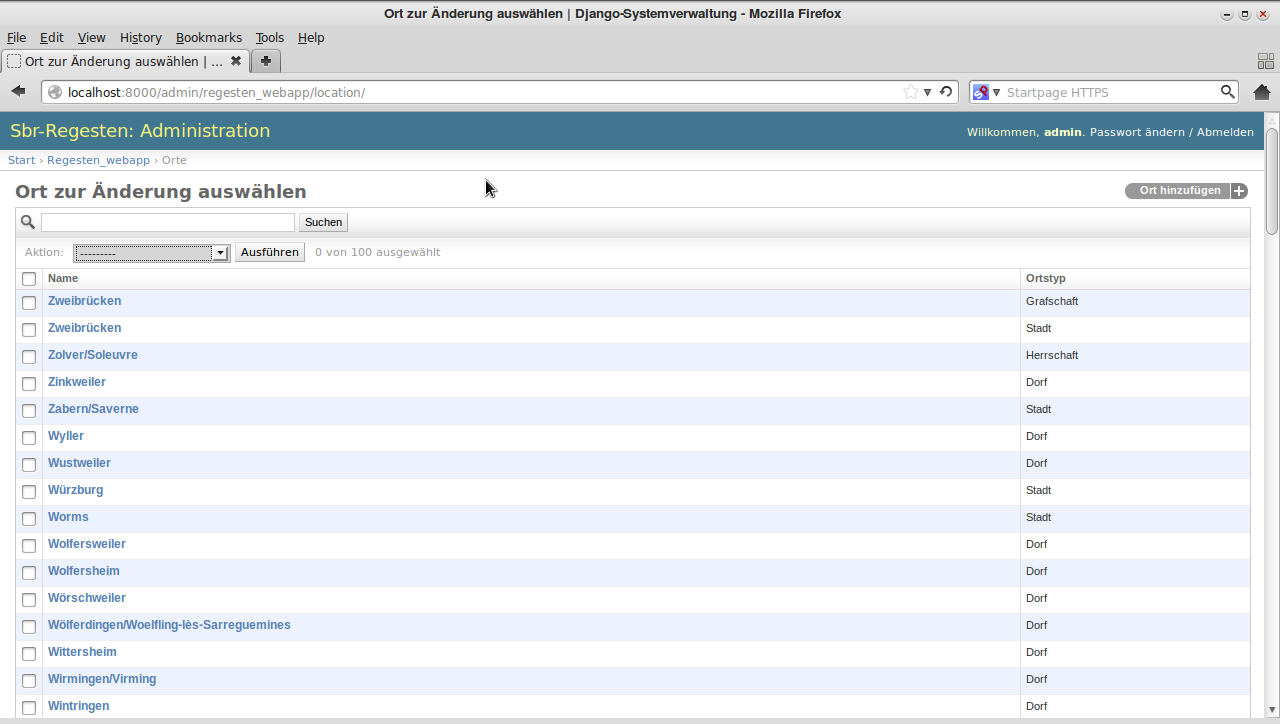
\includegraphics[scale=0.3]{img/admin-loc-listing}
  \caption{Example listing of database entries}
  \label{fig:admin-loc-listing}
\end{figure}

To sort the table by a specific column, click on its header. Clicking
more than once will toggle between ascending and descending order for
that column.

If you are looking for a specific entry, you can narrow down the list
by entering appropriate search terms in the search field and clicking
the \emph{Suchen} button. On the result page, click on the link next
to the information about the number search results to get back to the
full listing.

Note that for efficiency reasons, search is configured to consult only
a limited number of model fields for each entity.

\paragraph{Adding Data}
Starting from the main page of the admin interface, you can manipulate
the data in the database in various ways. For each entity/model that
has been configured to be editable via the admin interface, Django
displays two buttons; one for adding a new database entry for a
specific model (\emph{Hinzufügen}), and another one for changing
information associated with existing entries (\emph{Ändern}).

To add a new database entry for a specific model, click on the
corresponding \emph{Hinzufügen} button. This brings up the appropriate
input form for the model. For instance, the (top part of the) form for
adding a new Regest entry to the database looks like this:

\begin{figure}[h]
  \centering
  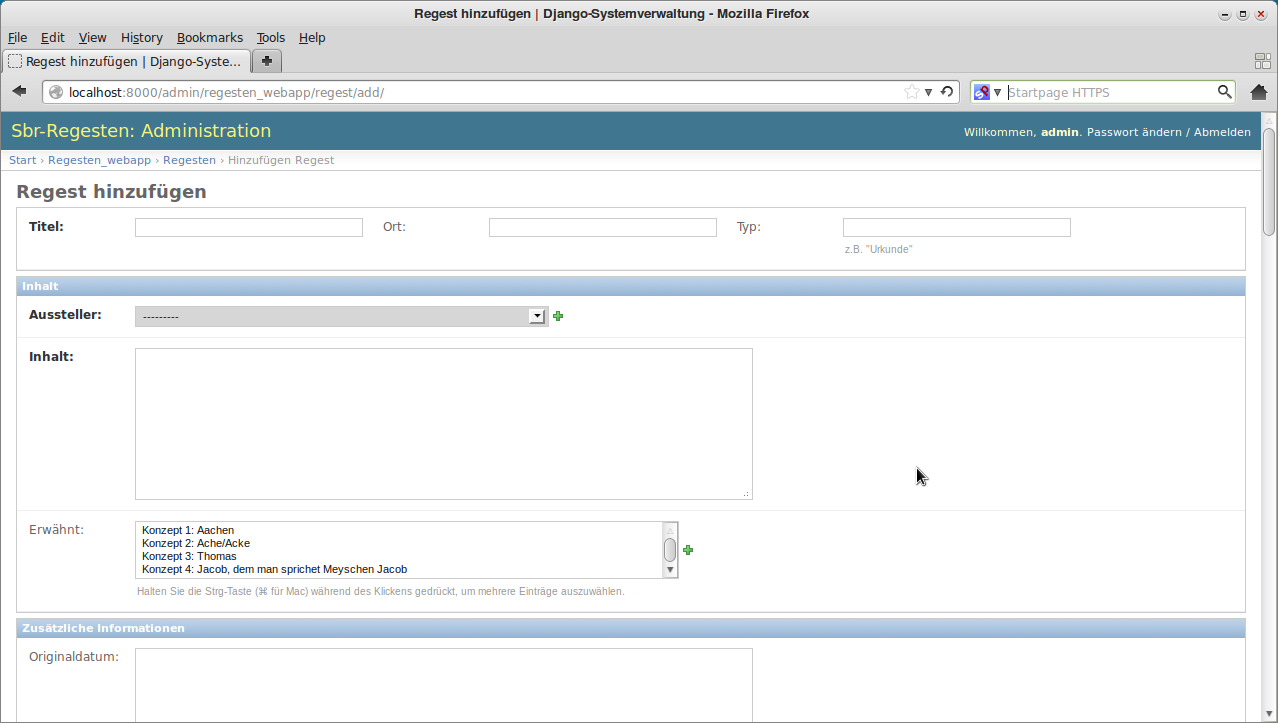
\includegraphics[scale=0.3]{img/add-regest}
  \caption{Example interface for adding a new entry to the database}
  \label{fig:add-regest}
\end{figure}

In any input form, fields with labels in bold font are mandatory. This
means that Django will not allow you to save a new entry to the
database without filling them in. Instead, it will annotate the fields
you failed to fill in with appropriate error messages and redisplay
the input form\footnote{The interface behaves in exactly the same way
  if you \textbf{edit} the information for an existing entry and
  (accidentally) delete any mandatory information.}:

\begin{figure}[h]
  \centering
  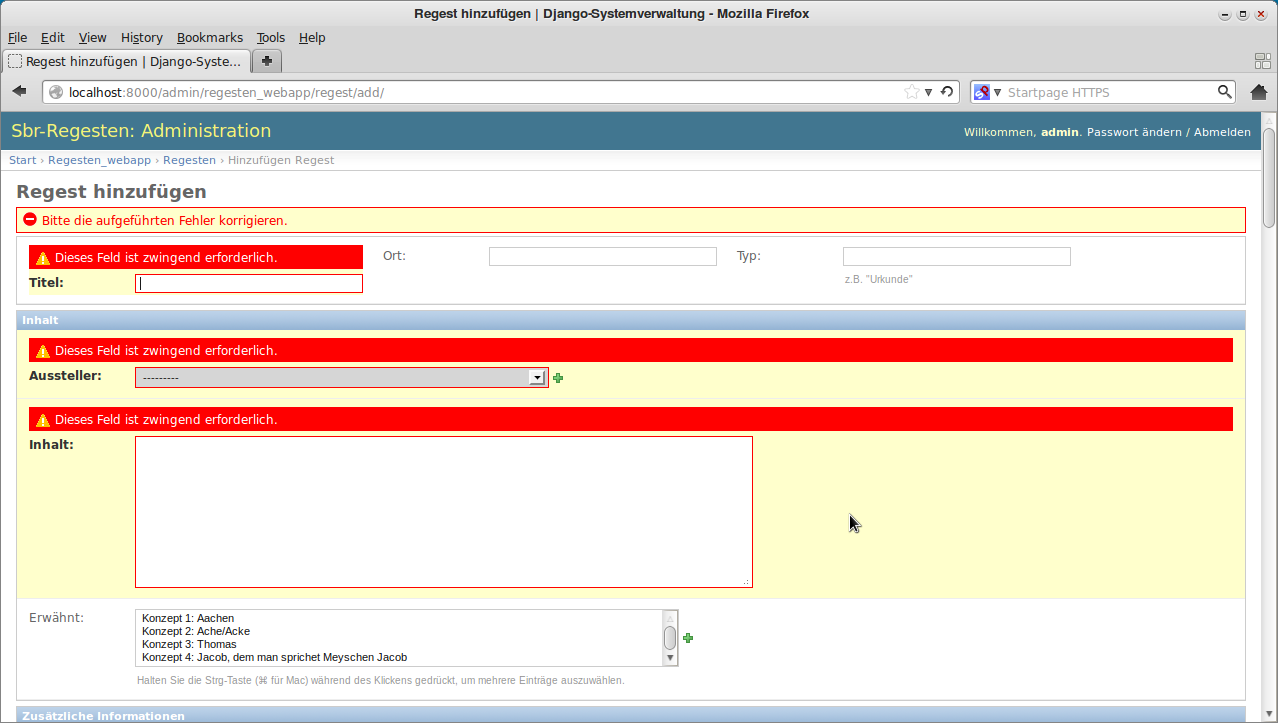
\includegraphics[scale=0.3]{img/add-regest-fail}
  \caption{Input form with errors}
  \label{fig:add-regest-fail}
\end{figure}

When you are done filling in the information that you would like to
store as a new entry in the database, click the \emph{Sichern} button
at the very bottom of the input form. This will take you back to the
listing of existing entries for the model that you were working on.
Alternatively, if you want to add another database entry for the same
model, click the \emph{Sichern und neu hinzufügen} button. This will
bring up a new input form for the same model. If you want to save the
entry and continue working on it afterwards, click \emph{Sichern und
  weiter bearbeiten}.\footnote{Note that this won't work if any of the
  mandatory fields are empty.}

If you are familiar with the Sbr-Regesten, most of the fields included
in the input forms for the different models should be
self-explanatory. Some of the less obvious fields are annotated with
examples of the type of input that they expect. However, before
starting to add or edit information from the admin interface, please
refer to chapter \ref{sec:data-model} to get a more detailed
understanding of the type of information represented by any given
field.

\paragraph{Manipulating Data}
The steps that are involved in editing existing data are very similar
to the ones that are required for adding new entries. On the main page
of the admin interface, click on the \emph{Ändern} button that
corresponds to the type of model you would like to edit one or more
entries for. This will bring up the already familiar listing of
database entries for the model. If necessary, sort or narrow down the
list as described above, then click on the name of the entry you would
like to edit. The fields of the input form that comes up will be
prepopulated with the information that is available for this entry.
Other than that it looks and behaves exactly like the form you are
already used to for adding new entries.

To get a list of all changes that were made to a specific database
entry via the admin interface, click on the button that says
\emph{Geschichte} in the top right corner of the input form.

\paragraph{Removing Data}
If you want to remove a specific entry from the database, navigate to
its input form as described above. Then, on the very bottom of the
page, click the \emph{Löschen} button. This will bring up a
confirmation page that looks like this:

\begin{figure}[h]
  \centering
  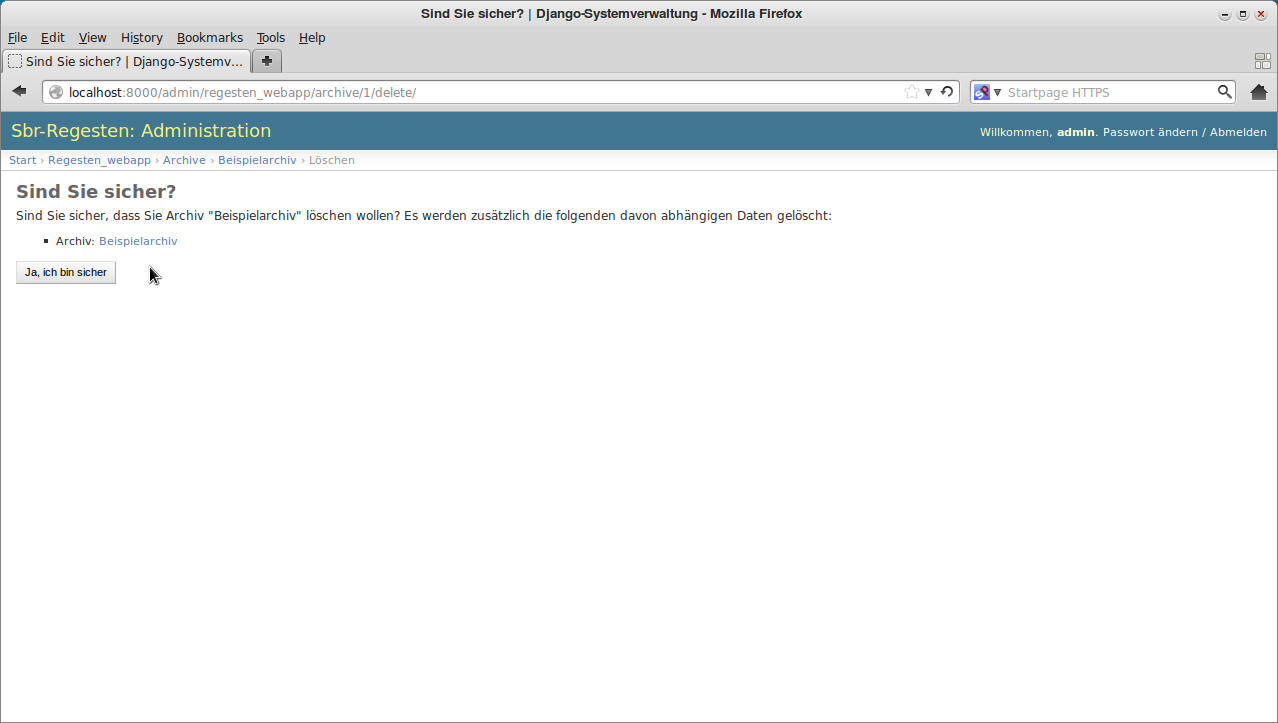
\includegraphics[scale=0.3]{img/confirm-delete}
  \caption{Confirmation page for deleting items}
  \label{fig:confirm-delete}
\end{figure}

Click on the \emph{Ja, ich bin sicher} button to finalize the action.
If you change your mind, you can use e.g. the breadcrumbs to navigate
somewhere else.

It is also possible to delete multiple entries at once. On the page
that lists all existing entries for a given model, mark the entries
you would like to delete by clicking on the checkboxes next to the
names of the entries. Then choose \emph{Ausgewählte MODEL\_NAME
  löschen} from the drop-down menu labeled \emph{Aktion} at the top
and click the \emph{Ausführen} button:

\begin{figure}[h]
  \centering
  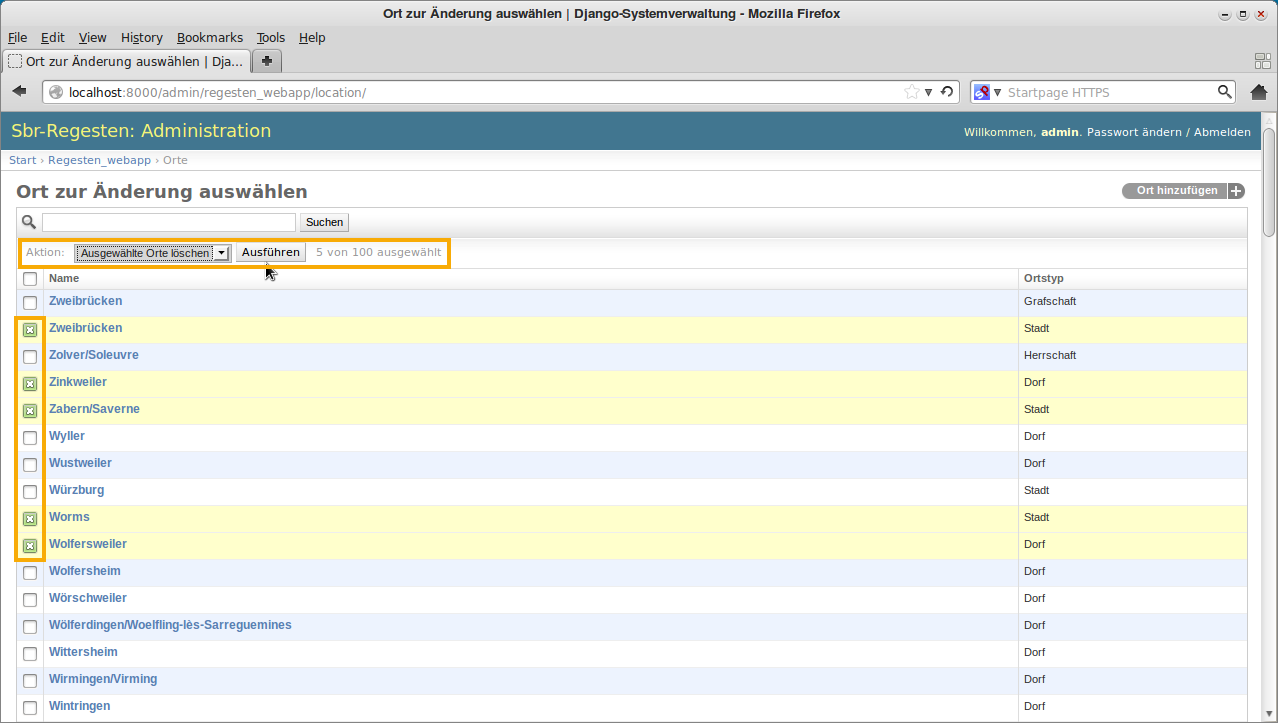
\includegraphics[scale=0.3]{img/delete-multiple}
  \caption{Deleting multiple items at once}
  \label{fig:delete-multiple}
\end{figure}

\subsection{Deployment}
\label{sec:deploy}

As mentioned in section \ref{sec:use}, the \texttt{runserver} command
runs the \emph{development} server for the Sbr-Regesten Web
Application. There are some additional steps you need to take to get
the application set up and running on a production server. Depending
on the type of server you are running, there are several ways to
achieve this, so when you are ready to deploy the application, please
consult the
\href{https://docs.djangoproject.com/en/1.4/howto/deployment/}{Deploying
  Django} section of the Django documentation for detailed information
on different ways to get the application running on your server.

\subsection{Extending the Web Application}
\label{sec:extend}

This section provides information about how to obtain a copy of the
source code for development purposes that includes the complete
history of changes. It also includes information about translating the
application, as well as some suggestions about missing features that
should be implemented next.

\subsubsection{Version Control with Git}
\label{sec:git}

\subsubsection{Next Steps: Suggestions for Future Extensions}
\label{sec:next}

\subsubsection{Internationalization: Translating the Application}
\label{sec:translate}

\subsection{Django Data Model}
\label{sec:data-model}
